% TPLAB 2

\documentclass[11pt,a4paper]{report}
\usepackage[utf8]{inputenc}
\usepackage{amsmath}
\usepackage{graphicx}
\usepackage{tabularx}
\usepackage{hyphsubst}

\usepackage{silence}
\WarningFilter{latex}{`h' float specifier changed to `ht'}

\makeatletter\let\l@spanish\l@nohyphenation\makeatother
\usepackage[spanish]{babel}
\usepackage{lipsum}
\usepackage{csquotes}
\usepackage{comment}
\usepackage{imakeidx}
\usepackage{multirow}
\usepackage{xcolor}
\usepackage[margin=2cm]{geometry}
\usepackage[hidelinks]{hyperref}
\usepackage[toc,acronym,nopostdot,nonumberlist]{glossaries}
\usepackage{titling}
\usepackage{tikzpagenodes}
\usepackage[ddmmyyyy]{datetime}
\usepackage{setspace}
\usepackage{indentfirst}
\selectlanguage{spanish}
\usepackage{float}
\usepackage{titlesec}
\usepackage{makecell}
\usepackage{listings}
\usepackage{biblatex}
\addbibresource{ref.bib}


\title{2}
\author{Bruno Glecer}
\date{\today}

% The preamble ends with the command \begin{document}
\begin{document} % All begin commands must be paired with an end command somewhere

\sloppy
\hbadness=99999

\pagenumbering{roman}
\begin{titlepage}
\begin{tikzpicture}[remember picture,overlay,shift={(current page.center)}]
\node[anchor=center,yshift=9cm]{
\includegraphics[scale=0.2]{figs/logo_utn.png}};
\end{tikzpicture}

\titleformat{\subsection}[runin]{}{}{}{}[]

\centering
\vspace{7cm}
\huge Informe de la práctica de laboratorio \#2 realizado para la materia Teoría de Circuitos 2\\
\vspace{2cm}


\Large Bruno Glecer\\
\vspace{2cm}
\large Materia dictada por\\
\large Mariano Llamedo Soria\\
\vspace{2cm}
\newdateformat{daymonthyear}{\THEDAY\ \monthname[\THEMONTH], \THEYEAR}
\daymonthyear\today \\
\vspace{1cm}
%December, 2019
%\large v2.3
\end{titlepage}



\pagenumbering{arabic}

%%%%%%%%%%%%%%%%%%%%%%%%%%%%%%%%%%%%%%%%%%%%%%%%%%%%%  
\chapter*{\centering\Large\bfseries Introducción}

Este informe trata de la práctica de laboratorio realizado el 12 de Octubre de 2023 para la materia Teoría de Circuitos II en el curso R4001 dictada por Mariano Llamedo Soria en la Facultad Regional de Buenos Aires de la Universidad Tecnológica Nacional. La preparación y realización del laboratorio fue realizada por el equipo constituido por: Bruno Glecer (autor del informe), Santiago Palozzo y Axel Nahum. Este trabajo tuvo la finalidad de llevar a la práctica los temas de filtrado digital vistos en clase. Mas específicamente, los conceptos de diseño de filtros FIR con los métodos algorítmicos de cuadrados mínimos y equiripple, y diseño de filtros IIR utilizando métodos tradicionales, pero aún así utilizando software para su síntesis.

\tableofcontents

%%%%%%%%%%%%%%%%%%%%%%%%%%%%%%%%%%%%%%%%%%%%%%%%%%%%%  
\newgeometry{left=0.8in,right=0.8in,top=0.3in,bottom=0.5in}


\chapter{Consigna}

La consigna de este trabajo práctico consiste en el diseño e implementación de tres filtros digitales: dos filtros FIR, y un filtro IIR, sobre el microcontrolador LPC1769, haciendo uso del ADC y DAC interno.

El código en su mayoría ya fue provisto por los docentes de la materia, este ya tiene implementado el procesamiento de la señal utilizando la librería de DSP del fabricante del microcontrolador.

Los filtros para implementar son los siguientes:

\vspace{0.5cm}

\begin{tabular}{|c|c|c|c|c|c|}
    \hline
    Filtro & Tipo
    & \makecell{Frecuencia \\ de corte}
    & \makecell{Frecuencia \\ de stop}
    & \makecell{Atenuación máxima \\ en banda de paso}
    & \makecell{Atenuación mínima \\ en banda de stop}\\
    \hline
    A & FIR Equiripple & 1 kHz & 2 kHz & 1 dB & 20 dB \\
    \hline
\end{tabular}

\vspace{0.5cm}

\begin{tabular}{|c|c|c|c|c|c|}
    \hline
    Filtro & Tipo
    & \makecell{Frecuencias \\ pass band}
    & \makecell{Frecuencias \\ stop band}
    & \makecell{Atenuación \\ pass band}
    & \makecell{Atenuación \\ stop band} \\
    \hline
    B & \makecell{FIR Least \\ Squares} & 2 a 8 kHz & 4 a 6 kHz & 1 dB & 20dB \\
    \hline
\end{tabular}

\vspace{0.5cm}


\begin{tabular}{|c|c|c|c|c|c|}
    \hline
    Filtro & Tipo
    & \makecell{Frecuencia \\ de corte}
    & \makecell{Frecuencia \\ de stop}
    & \makecell{Atenuación máxima \\ en banda de paso}
    & \makecell{Atenuación mínima \\ en banda de stop}\\
    \hline
    C & \makecell{IIR \\ Butterworth} & 2 kHz & 3 kHz & 1 dB & 20 dB \\
    \hline
\end{tabular}

\vspace{0.5cm}


Estos filtros son implementados con una frecuencia de muestreo de $F_s = 44.1 \mathrm{kHz}$

 
Una vez calculados los coeficientes, estos tienen que ser copiados al código en forma de arrays, compilado y subido al microcontrolador. También será necesario implementar dos filtros analógicos: un filtro antialiasing en la entrada del ADC, y un filtro de interpolación en la salida del DAC.

Para evaluar el comportamiento del filtro se utilizaron dos métodos: Primero, utilizando un generador de tensiones le aplicamos una señal senoidal en la entrada, y utilizando un osciloscopio en el que visualizamos la señal de entrada y salida simultáneamente, obtuvimos la ganancia. Una vez completado esto, utilizamos un analizador de audio para obtener una medición más automatizada y precisa de la respuesta en frecuencia.
Además de medir la respuesta en frecuencia de cada filtro, medimos la respuesta en frecuencia cuando el filtro digital se anula y remplaza por un "talkthrough" digital, que se puede pensar como un filtro con ganancia unitaria y fase cero.

\chapter{Cálculos}

\lstset{language=C,keywordstyle={\bfseries \color{blue}}}

\section{Cálculos de coeficientes}

Para calcular los coeficientes de los filtros, utilizamos la librería SciPy para Python. El jupyter notebook con el código para el diseño se encuentra subido en el repositorio del trabajo práctico. \cite{notebook_calculos}

\vspace{0.5cm}


Para el cálculo del primer filtro (A: FIR Equiripple) utilizamos la función \texttt{scipy.signal.remez} que recibe las frecuencias de las bandas y sus ganancias deseadas para generar los coeficientes.
Utilizamos 151 coeficientes (o "taps") para este filtro.

\vspace{0.5cm}

Para el cálculo del segundo filtro (B: FIR Least Squares) utilizamos la función \texttt{scipy.signal.firls}, que tiene un comportamiento muy similar al \texttt{remez} excepto que aproxima los coeficientes utilizando el método de cuadrados mínimos.
Al igual que para el filtro A, utilizamos 151 taps.

\vspace{0.5cm}

Para el cálculo del último filtro (C: IIR Butterworth) utilizamos la función \texttt{scipy.signal.iirdesign} que recibe las frecuencias de corte, ganancias y el tipo de filtro (Butterworth, Chebyshev, etc.) para generar los coeficientes del numerador y denominador de un filtro IIR.
Es importante exportar los filtros como varias etapas de segundo orden, para esto utilizamos el argumento opcional \texttt{output=sos} de la función. También es importante redistribuir la ganancia entre las etapas para asegurar estabilidad. Esto está implementado directamente en el código, previo a la impresión de los valores.
Esta implementación resultó en la generación de 4 etapas de segundo orden.

Una vez calculados los coeficientes, estos fueron cargados como constantes al código del microcontrolador. Este se encuentra disponible en el repositorio del trabajo práctico \cite{codigo}

\section{Filtros de acondicionamiento de señal}

La frecuencia de muestreo del filtro es de $F_s = 44.1 \mathrm{kHz}$, entonces la frecuencia de Nyquist será de $F_s = 22.05 \mathrm{kHz}$. La frecuencia más alta especificada en cualquiera de los filtros es de 8kHz (en el filtro B). Entonces, en teoría, podemos utilizar filtros pasa bajos con frecuencias de corte entre 8kHz y 22.05kHz. Por simplicidad, decidimos diseñar los filtros en base a un capacitor de 10nF y una resistencia de 1k$\Omega$, lo cual resulta en un filtro con una frecuencia de corte de: $f_c = \frac{1}{2 \pi R C} = 15.9\mathrm{kHz}$ 
Esta frecuencia de corte nos pareció apropiada para esta aplicación.

\begin{figure}[h]
    \centering
    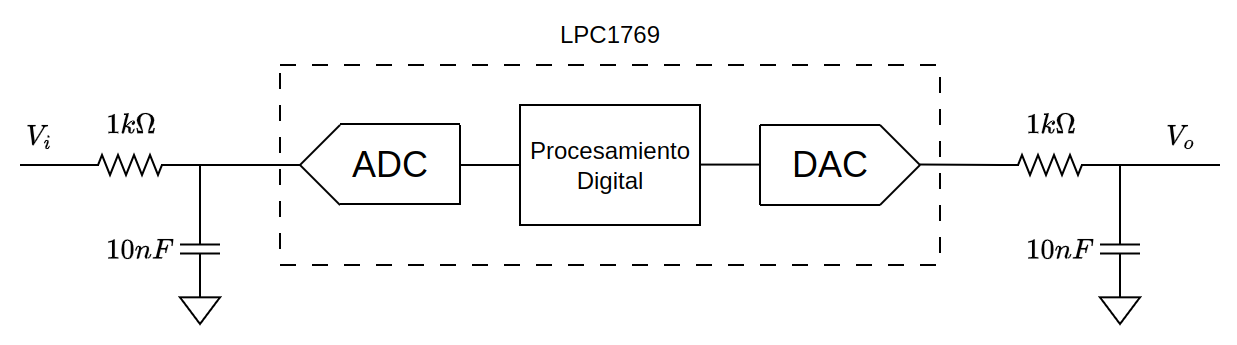
\includegraphics[scale=0.4]{figs/filtro_sch.png}
    \caption{Esquemático del filtro digital en cascada con el filtro antialias y de interpolación}
\end{figure}

\chapter{Armado del filtro}

Para utilizar el LPC1769, utilizamos la placa de desarrollo de Embedded Artists. Esta fue montada sobre un protoboard, junto con los filtros RC en las entradas y salidas. Debido a que las frecuencias que se trabajan son relativamente bajas, no creemos que el uso de un protoboard cause problemas.



\begin{figure}[h]
    \centering
    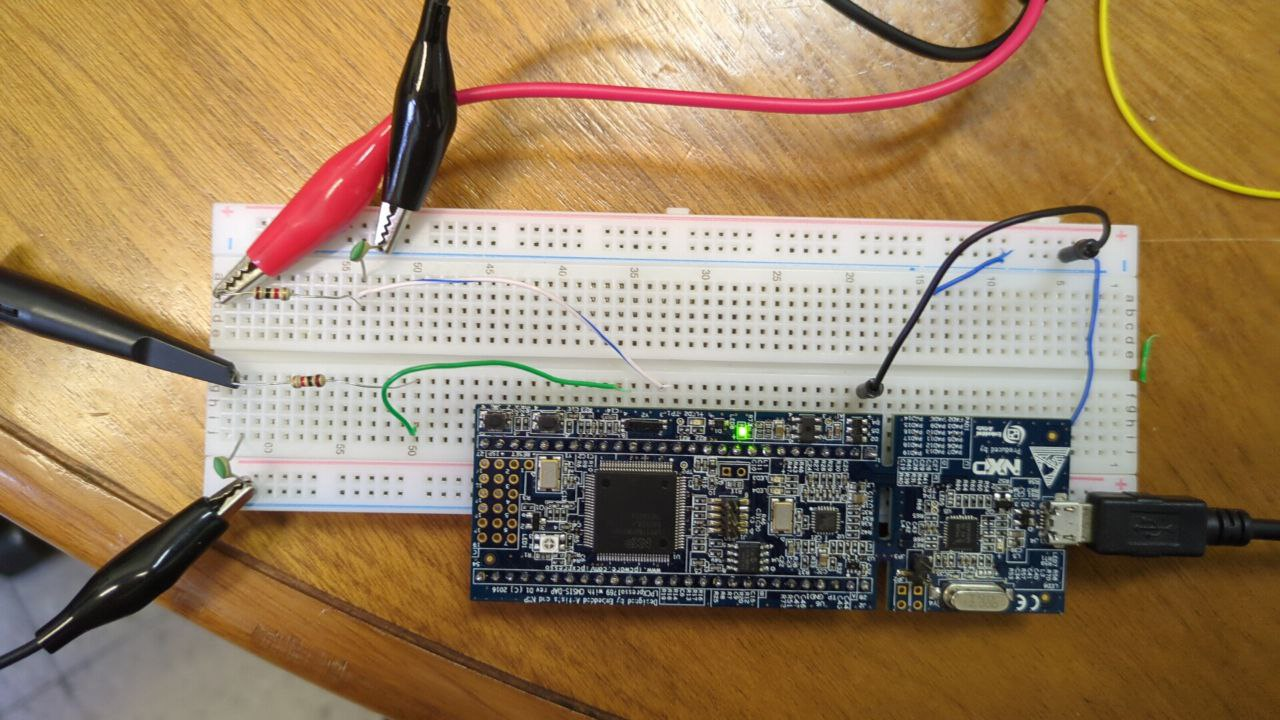
\includegraphics[scale=0.25]{figs/filtro_armado.jpg}
    \caption{Filtro armado sobre el protoboard}
\end{figure}

Desafortunadamente, una vez que el filtro fue armado y configurado en modo talkthrough, en la salida del circuito se podían observar pequeños pulsos con una ocurrencia aleatoria como se muestran en la siguiente figura:

\begin{figure}[h]
    \centering
    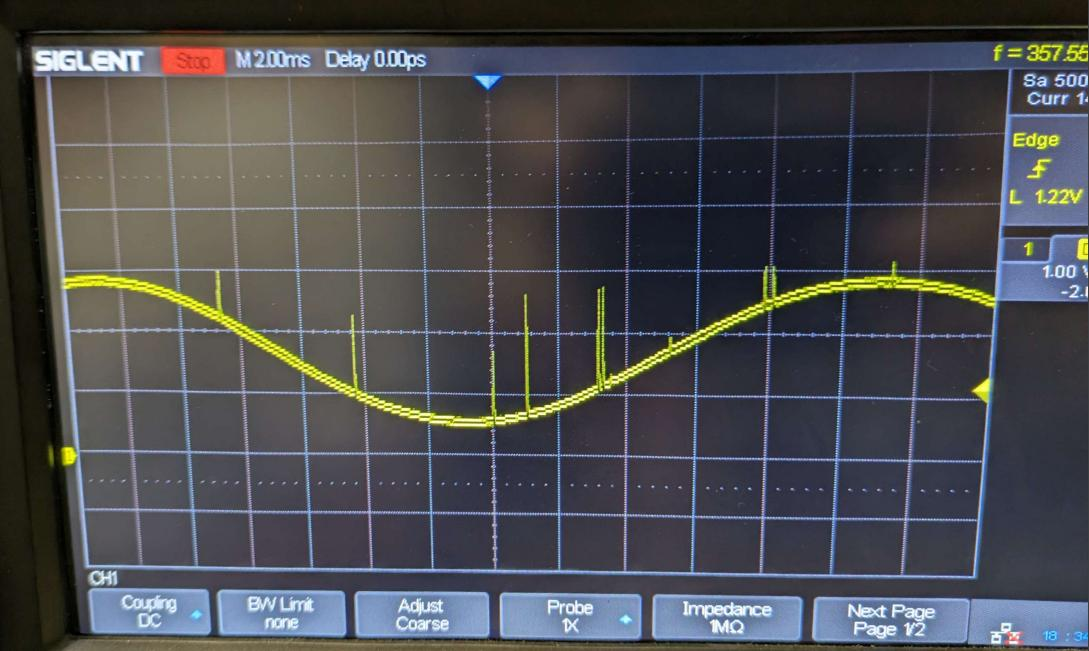
\includegraphics[scale=0.4]{figs/ruido.jpg}
    \caption{Ruido en la señal de salida}
\end{figure}

Depurando el programa, pudimos identificar que esos pulsos eran causados por el ADC. Creemos que es una falla propia del microcontrolador, ya que todos nuestros compañeros y otros usuarios en los foros online de NXP también observaban el mismo tipo de ruido en distintas situaciones. No logramos encontrar una forma de resolverlo sin cambiar sustancialmente el código.

\chapter{Mediciones}

Para la medición con osciloscopio utilizamos un generador de funciones para generar una señal senoidal con tensión pico a pico de 3V. La frecuencia la íbamos decidiendo en el momento para cada filtro dependiendo de donde se encuentren las frecuencias críticas. Para cada frecuencia se midió la tension RMS de entrada y salida, y calculamos su relación para obtener la ganancia.
El generador de funciones tiene una resistencia de salida de 50$\Omega$, pero esta no deberia tener un efecto medible en el sistema debido a la alta resistencia de entrada del filtro (\textgreater 1k$\Omega$)



\begin{figure}[h]
    \centering
    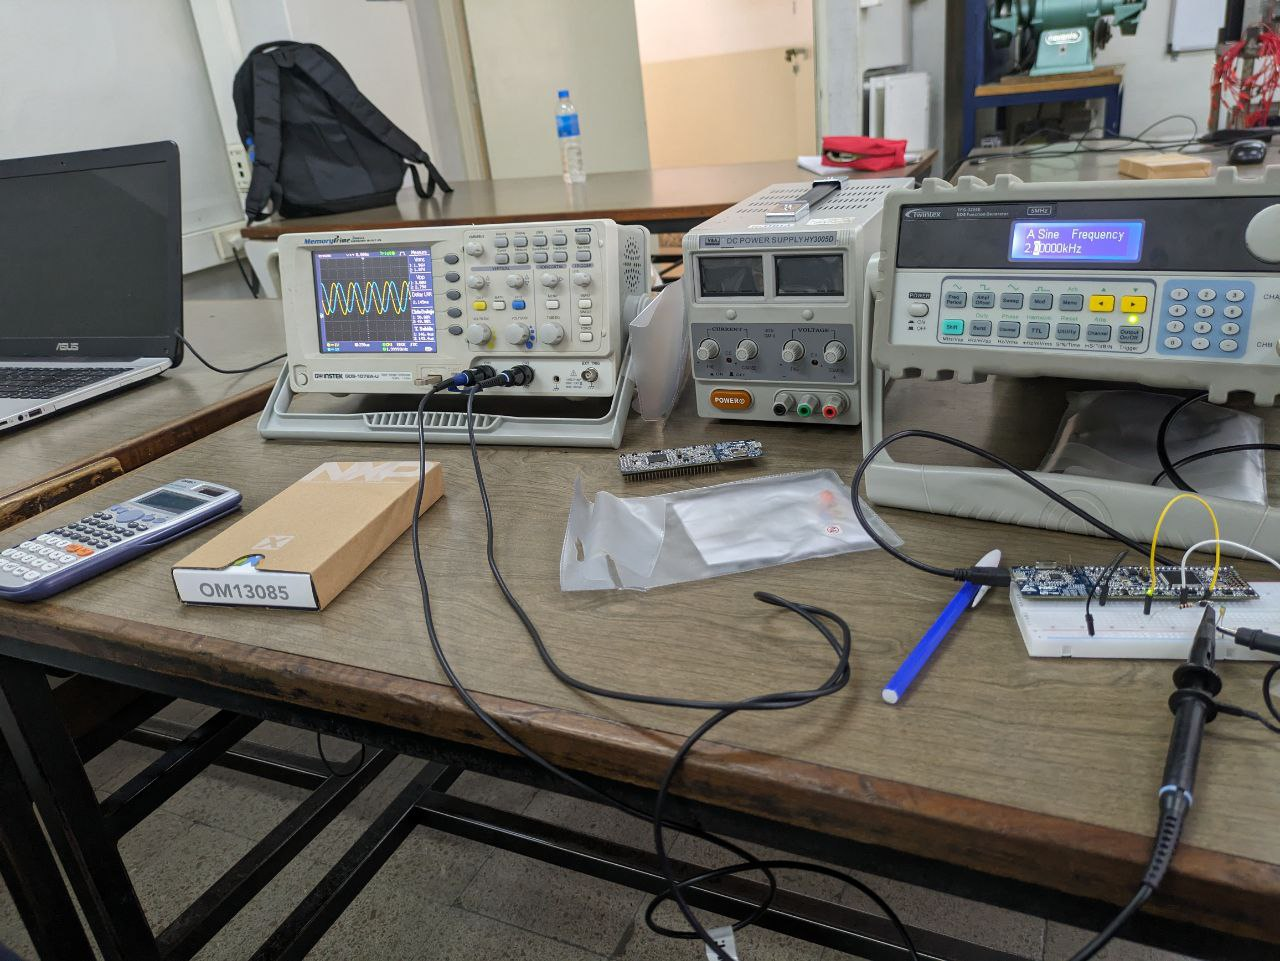
\includegraphics[scale=0.3]{figs/setup.jpg}
    \caption{Setup de medición con osciloscopio y generador de funciones}
\end{figure}

\pagebreak

\section{Talkthrough}

\begin{figure}[h]
    \centering
    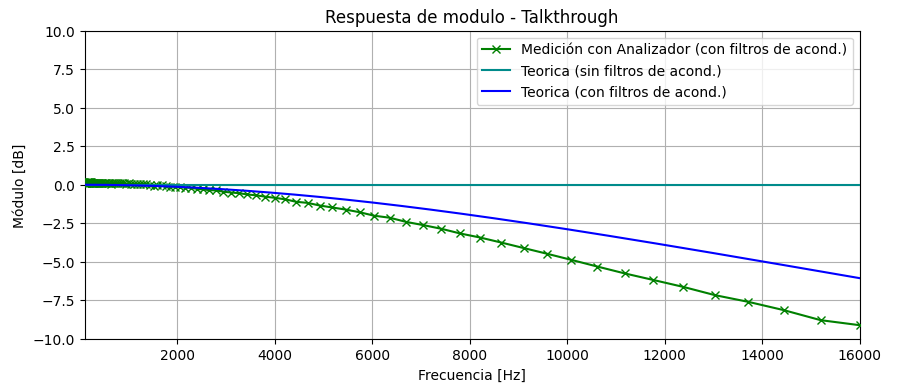
\includegraphics[scale=0.7]{figs/talkthrough.png}
    \caption{Medición de talkthrough}
\end{figure}

Las mediciones del talkthrough fueron solamente realizadas con el analizador de audio. Los resultados son similares a los esperados, los filtros de acondicionamiento afectan las altas frecuencias, pero inevitablemente atenúa en cierto nivel las frecuencias en el rango que operarán los filtros. Como se comentó anteriormente, la frecuencia más alta de interés es de 8kHz. En este punto, la atenuación causada por los filtros es de alrededor de 3dB.

Se puede ver una discrepancia entre la atenuación medida y la predicción con el análisis de los filtros RC. Esto se puede deber a varios factores, incluyendo limitaciones del microcontrolador, tolerancias de los valores de los componentes (especialmente los capacitores), el ruido que se observó anteriormente entre otras.

\section{Filtro A: FIR Equiripple}

\begin{figure}[h]
    \centering
    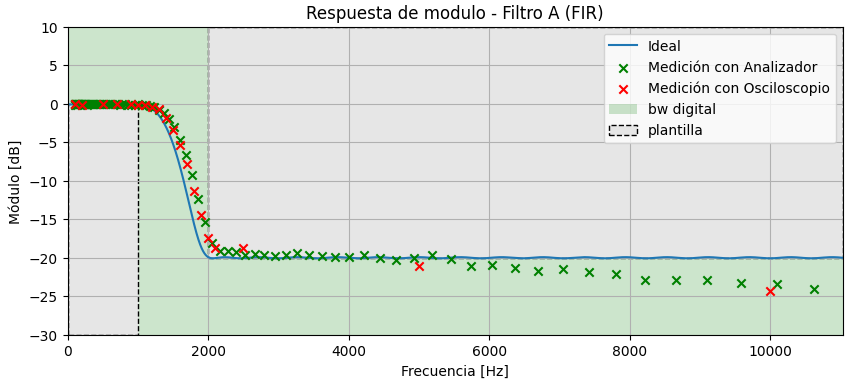
\includegraphics[scale=0.7]{figs/filtro_a.png}
    \caption{Medición de módulo del filtro A}
\end{figure}

El funcionamiento del filtro A aparenta ser muy bueno. La frecuencia de corte corresponde muy bien con la esperada, y parece cumplir adecuadamente con la plantilla. Las mediciones con el osciloscopio y el analizador de audio también resultaron muy cercanas. Para las frecuencias superiores a 6kHz se puede empezar a observar el efecto de los filtros de acondicionamiento.


\section{Filtro B: FIR Least Squares}

\begin{figure}[h]
    \centering
    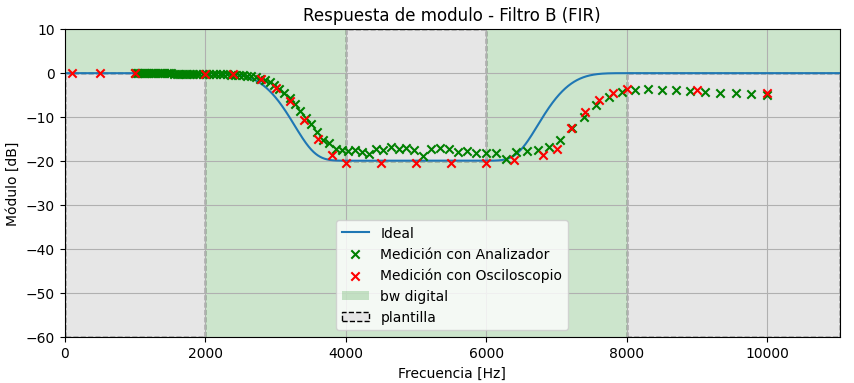
\includegraphics[scale=0.7]{figs/filtro_b.png}
    \caption{Medición de módulo del filtro A}
\end{figure}


El filtro B aparenta funcionar bien en general, pero se puede ver que hay diferencias en ambas de las frecuencias de corte, en especial en la superior. También se puede ver que la atenuación en la banda de stop es ligeramente baja. Sospechamos que esto se puede deber a problemas con el timing interno del microcontrolador. Si deseamos que la plantilla se cumpla más estrictamente, se puede utilizar una atenuación más alta en la banda de stop y más baja en las bandas de paso.


\section{Filtro C: IIR Butterworth}

\begin{figure}[h]
    \centering
    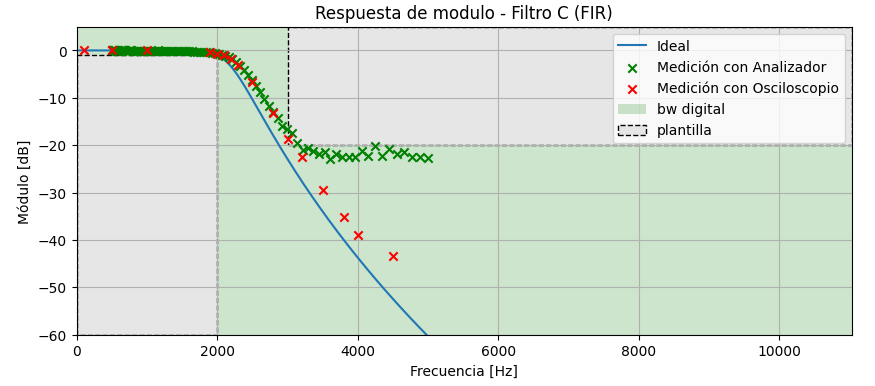
\includegraphics[scale=0.7]{figs/filtro_c.png}
    \caption{Medición de módulo del filtro C}
\end{figure}

El filtro C aparenta funcionar bien y cumplir con la plantilla. Igualmente, se puede observar una discrepancia inesperada entre las mediciones con el analizador de audio y el osciloscopio. Sospechamos que se debe a limitaciones del rango dinámico del analizador, en el que no puede medir correctamente señales por debajo de -20dB. También puede deberse a la interferencia causada por el ruido del ADC remarcado anteriormente.

El notebook en donde se realizaron los gráficos anteriores se encuentra disponible en el repositorio del trabajo práctico. \cite{notebook_analisis}

\chapter{Conclusiones}

Este trabajo práctico nos sirvió para llevar a la práctica los conceptos de filtrado digital que fueron vistos en clase, en particular los distintos métodos de síntesis de filtros FIR y IIR, y como podrían ser implementados en un microcontrolador. Esto último nos pareció particularmente interesante debido a que nos encontramos con el problema del ruido en la salida que, a pesar de no haber logrado solucionarlo, logramos identificar el origen del problema.

El código del microcontrolador también nos resultó interesante, en particular el método de buffers ¨Ping pong" que se utilizó para implementar los filtros y el uso de la librería nativa del microcontrolador para hacer uso del hardware de DSP que tiene el dispositivo.


En cuanto a los resultados, estos no fueron tan buenos como esperados y hubo discrepancias grandes entre lo ideal y lo medido, al menos en comparación con el trabajo práctico anterior de filtros analógicos. A pesar de esto, estuvimos satisfechos con el rendimiento de los filtros y creemos que se pueden mejorar si se refinan los parámetros de diseño, o si se utilizan filtros de acondicionamiento de mayor orden. 


\printbibliography[title={Referencias}]


\end{document}